\documentclass[final,5p,times,twocolumn,authoryear]{elsarticle}
\usepackage{amsmath,amssymb,amsthm}
\usepackage{booktabs}
\usepackage{graphicx}
\usepackage{etoolbox}
\usepackage{multirow}
\usepackage[colorlinks=true,linkcolor=blue,citecolor=blue,urlcolor=blue]{hyperref}
\AtBeginEnvironment{table}{\small\setlength{\tabcolsep}{4pt}}
\AtBeginEnvironment{table*}{\small\setlength{\tabcolsep}{4pt}}
\newcommand{\fitc}[1]{\resizebox{\ifdim\width>\columnwidth\columnwidth\else\width\fi}{!}{#1}}
\newcommand{\fitw}[1]{\resizebox{\ifdim\width>\textwidth\textwidth\else\width\fi}{!}{#1}}
\graphicspath{{fig/261001/}}
\newtheorem{proposition}{Proposition}
\newcommand{\SOL}{\mathcal{S}}
\newcommand{\FORCED}{\textsc{forced}}
\newcommand{\FREE}{\textsc{open}}
\makeatletter\def\thefnote{\ifcase\c@fnote\or$\dagger$\or$\ddagger$\fi}\makeatother
\journal{Swarm and Evolutionary Computation}

\begin{document}
\begin{frontmatter}

\title{Exact Posteriors for Values, Exact Costs for Choices:\\
Two-Stage Learned Branching for Binary Linear Systems}

\author[ku]{Gwang-Jong Ko\corref{cor1}}
\author[ku]{Taesu Cheong\fnref{fn1}}
\author[ku]{In-Chan Choi\fnref{fn1}}
\cortext[cor1]{Corresponding author.}
\fntext[fn1]{Footnote text for the \dag{} mark to be supplied by the authors.}
\affiliation[ku]{organization={School of Industrial and Management Engineering, Korea University},
                city={Seoul},
                country={Republic of Korea}}

\begin{abstract}
A binary linear system (BLS) asks for $\mathbf{x}\in\{0,1\}^n$ with $A\mathbf{x}=\mathbf{b}$ for a $0/1$ matrix $A$. The problem has no objective, its linear relaxation carries little information on the instances that arise in practice, and unit propagation is inert near the root of a search tree, so a complete search is decided by its branching choices. We present a branching heuristic for the depth-first search of a BLS that is learned in two stages from two exact signals. Stage~1 learns \emph{which value} to try first: on instances small enough to enumerate every solution, the conditional marginal $\Pr[x_j{=}1\mid A,\mathbf{b},\text{partial assignment}]$ is exact, and because conditioning a BLS on a partial assignment is the same as reducing it, a single graph network trained on reduced instances predicts at every node of the tree. Stage~2 learns \emph{which variable} to branch on: the cost of a decision, the number of nodes its subtree expands, is produced exactly by the search, and an actor-critic fine-tuning on that cost, started at the Stage-1 rule with the marginal network frozen, changes only the branching order. The deployed solver runs lattice reduction first and the guided search on what it leaves. On $100$ instances of size $21\times60$ with matched wall-clock budgets and three seeds, Stage~1 expands $5.5\times$ fewer nodes than LP-guided branching and is $2.0$--$2.3\times$ faster; Stage~2 removes a further $2.3$--$2.4\times$ of the nodes and $2.0$--$2.4\times$ of the time ($p<0.001$), replicates across training seeds, and transfers to sizes it never saw: at $24\times70$ the fine-tuned policies solve $30/30$ instances $2.3$--$3.3\times$ faster than Stage~1, and at $28\times80$ they double the solve rate within budget. Ablations show that the two signals are not interchangeable: raising the value accuracy of the marginal network where its margin lives enlarges the tree, while the cost-tuned policy branches on variables the network is \emph{less} sure about and shrinks it.
\end{abstract}

\begin{keyword}
Binary linear systems \sep Learning to branch \sep Exact conditional marginals \sep Reinforcement learning \sep Tree search \sep Graph neural networks
\end{keyword}

\end{frontmatter}

\section{Introduction}
\label{sec:intro}

A binary linear system (BLS) is the feasibility problem
\begin{equation}
\text{find } \mathbf{x}\in\{0,1\}^n \text{ such that } A\mathbf{x}=\mathbf{b},\qquad A\in\{0,1\}^{m\times n},\ \mathbf{b}\in\mathbb{Z}_{\ge0}^m,
\label{eq:bls}
\end{equation}
with solution set $\SOL$. It is the general form of a reconstruction task in laser-based non-destructive testing: a binary occupancy image must reproduce a set of integer projections exactly, the scanned object exists, so a solution exists and is often not unique, and the reconstruction has to keep pace with a production line. The instances that matter are dense, with right-hand sides near the middle of each row's range, and they are hard out of proportion to their size.

Three properties defeat the standard tools on such instances. There is no objective, so the bound-based pruning of branch-and-bound has nothing to work with. The linear relaxation is always feasible but carries little information: the relaxation polytope is wide, its vertices lie far from $\{0,1\}^n$, and rounding a vertex predicts a variable's value only slightly better than chance at the root. Unit propagation, the workhorse of constraint solvers, fires only when a row is saturated, which never happens at the root and rarely near it. The classical remedy for this family, lattice basis reduction, solves small instances outright but stops working as the size grows, and complete solvers with clause learning, while fast, do not make the branching decision itself any cheaper to get right. What is left to a complete search is the quality of its branching decisions, and that is the object of this paper.

A branching decision has two parts, and we show that they are best learned from two different exact signals. \emph{Which value} a variable should take first is a question about where the solutions are; on instances small enough to enumerate, the conditional marginal of $x_j$ given the assignments made so far answers it exactly. \emph{Which variable} to branch on is a question about the cost of what follows; the number of nodes the subtree expands answers it exactly, and the search produces that number as it backtracks. Stage~1 of our method trains a bipartite graph network on the first signal. A reduction identity (Proposition~\ref{prop:reduce}) makes the same network valid at every node of the tree, and the marginals partition the variables of a node into those whose wrong value empties the subtree ($\FORCED$) and those whose either value still reaches a solution ($\FREE$); only the former cost a backtrack, and their share grows steeply with depth, which is why the network is trained inside the tree. Stage~2 fine-tunes the branching order on the second signal with the Stage-1 network frozen, so that whatever improves can be attributed to the order alone. The deployed solver (Figure~\ref{fig:framework}) runs the classical lattice stage first and the guided search on what it leaves; the network only guides, so the search stays complete and a wrong prediction costs backtracking and nothing else.

\paragraph{Contributions.}
\begin{enumerate}
\item A branching heuristic for BLS learned from exact conditional marginals inside a complete search. The reduction identity that carries the target to every node, the $\FORCED$/$\FREE$ partition, and the finding that in-tree supervision is what makes learned guidance better than relaxation rounding (a network trained on root states is worse) are new.
\item A cost-aware fine-tuning of the branching order that starts from the posterior-derived rule and trains only the order. The starting point and the frozen marginal are what let the gain be attributed and what make it transfer to larger instances than it was trained on.
\item Evidence that the two signals capture different things: sharpening the value signal where its margin lives enlarges the tree, while the cost-tuned policy prefers variables the value model is less sure about and shrinks it.
\item A controlled evaluation with solution multiplicity matched across sizes, matched wall-clock budgets, an identical search loop for every branching rule, three evaluation seeds, two training seeds, a $100$-instance test set, comparisons against CP-SAT and SCIP, and the deployed cascade with lattice reduction in front.
\end{enumerate}

Section~\ref{sec:related} reviews related work and states what it leaves open for this problem, Section~\ref{sec:problem} states the problem and the reduction identity, Section~\ref{sec:method} the method, Section~\ref{sec:exp} the experiments, organised around four questions, and Section~\ref{sec:conclusion} concludes with the limitations and future work.

\begin{figure*}[t]
\centering
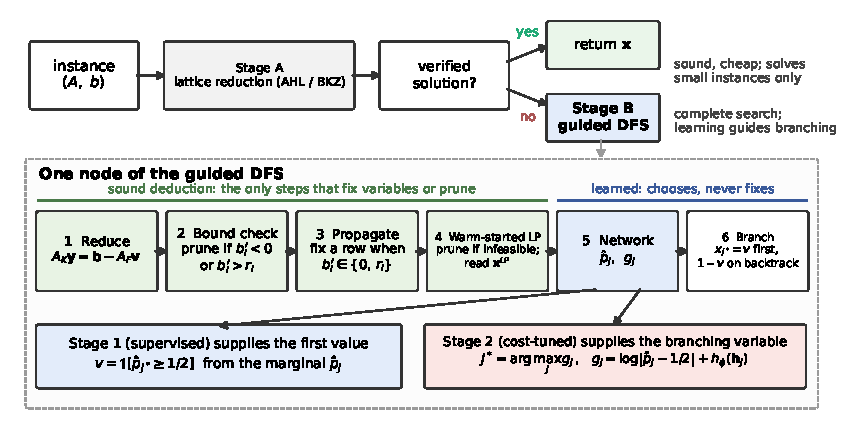
\includegraphics[width=\textwidth]{framework.pdf}
\caption{The deployed solver. Stage~A, lattice reduction, returns a verified solution when it finds one; Stage~B, the guided depth-first search, handles the rest. Inside a node, steps 1--4 are sound and are the only steps that fix variables or prune; the network at step 5 only chooses, the value from Stage~1 and the variable from Stage~2.}
\label{fig:framework}
\end{figure*}

\section{Related work}
\label{sec:related}

\paragraph{Marginals of the solution set as a branching signal.} Branching on the fraction of solutions that agree with a decision predates learning: counting-based search \citep{pesant2012counting} branches on the variable--value pair of maximum solution density computed inside individual constraints, and belief-propagation-guided decimation \citep{montanari2007solving} fixes the most biased variable under approximate marginals. NSNet \citep{li2022nsnet} trains a graph network on exact marginals of the satisfying assignments of a SAT formula, obtained by enumerating them, and rounds the estimates into an initial assignment for local search; MIP-GNN \citep{khalil2022mipgnn}, Neural Diving \citep{nair2020solving} and predict-and-search \citep{han2023gnn} predict per-variable biases from collected near-optimal solutions and use them to fix variables, warm-start or restrict a search. Stage~1 shares NSNet's target and differs in where and how it is used: the marginals are conditional and carried to every node of a complete search by the reduction identity, they guide branching without fixing anything, and the $\FORCED$/$\FREE$ partition and the controlled in-tree-versus-root comparison have no counterpart in that work.

\paragraph{Learning to branch.} \citet{khalil2016learning} and \citet{gasse2019exact} imitate strong branching, the latter with the bipartite variable--constraint graph network we also use; imitation targets an expert's ranking rather than the tree size the ranking is meant to reduce. Optimising tree size directly is the subject of a line of reinforcement-learning work: FMSTS \citep{etheve2020reinforcement} uses the size of a node's subtree as an observable Q-value, shows that under depth-first search minimising every subtree minimises the whole tree, and learns from scratch; tree MDPs \citep{scavuzzo2022learning} formalise the per-subtree credit assignment; retro branching \citep{parsonson2023reinforcement} learns from retrospectively extracted subtree trajectories; SORREL \citep{sorrel2025} initialises from demonstrations. Neuro\# \citep{vaezipoor2021learning} trains a graph network on the residual formula of a \#SAT solver by evolution strategies and generalises to larger instances. Stage~2 uses the FMSTS credit assignment with a plain policy gradient \citep{williams1992simple}; what it adds is the starting point and the scope, a rule derived from exact marginals, frozen, with only the branching order learned. The classical statements of the objective are the fail-first principle \citep{haralick1980increasing} and impact-based search \citep{refalo2004impact}. Value ordering has been learned in constraint programming from solutions \citep{chu2015learning} and by deep Q-learning \citep{cappart2021combining}; we take the value from the exact posterior and learn only the variable.

\paragraph{Market split, lattice methods and complete solvers.} The market split problem of \citet{cornuejols1999class} is the benchmark that exposes the weakness of branch-and-bound on systems like~\eqref{eq:bls}: $m$ equality rows over $n=10(m-1)$ binary variables, coefficients drawn uniformly from $\{0,\dots,99\}$, and each right-hand side set to half its row sum, so that the relaxation polytope is wide, its vertices far from integrality, and bounding prunes almost nothing; branch-and-cut stops at $m\approx7$. \citet{aardal2000diophantine,aardal2000market} solved these instances by reformulating them on a lattice: the Aardal--Hurkens--Lenstra embedding turns a solution into one of the shortest vectors of a lattice, LLL/BKZ reduction \citep{lenstra1982factoring,schnorr1994lattice} finds it, and the recovered vector is verified, so the method is sound. Lattice enumeration remains the state of the art on the benchmark: \citet{wassermann2025solving} solves QOBLIB market-split instances up to $m=14$ on one CPU. Our instances share the ingredients that make market split hard, dense rows and right-hand sides at the middle of their range, and differ in having $0/1$ coefficients, a planted solution and a search regime of up to $80$ variables; lattice reduction is therefore the natural first stage of a BLS solver, and our contribution begins where it stops working. Constraint solvers with clause learning \citep{marquessilva1999grasp,ohrimenko2009propagation} manufacture information as they descend and set the wall-clock reference we compare against. Direct satisfiability prediction has a weak record \citep{selsam2019neurosat,li2023g4satbench}, and message-passing networks provably cannot separate some feasible/infeasible pairs \citep{chen2023representing}. Both learned stages of our method are instances of amortised inference \citep{amos2023tutorial,gershman2014amortized}: the marginal network replaces one relaxation per variable, the cost head replaces a completed search.

\paragraph{What these approaches leave open for a BLS.} Four gaps shape the method. First, the marginal-based methods estimate marginals once, at the root or inside single constraints, and then fix variables; a feasibility problem with many solutions needs the marginals \emph{conditional} on the partial assignment at every node, and a use that keeps the search complete when the estimate is wrong. Second, learned branching for mixed-integer programming either imitates strong branching, which does not exist without an objective, or learns from scratch, which requires a per-decision credit that is well posed and a starting point that is not random; a BLS needs a cost signal that is exact per decision and an initialisation that is already a good rule. Third, lattice reduction is sound and cheap but its coverage collapses with size, so it must be combined with a search rather than replaced. Fourth, a network cannot be trusted with a verdict on feasibility, so it must never be asked for one. The method below takes the exact conditional marginal as the value signal, the exact subtree node count as the cost signal, the marginal rule as the starting point of the cost-tuned policy, and a cascade in which the network only guides.

\section{Problem statement and preliminaries}
\label{sec:problem}

\subsection{Instances and scope}
\label{sec:problem-instances}

We study feasible instances of~\eqref{eq:bls}: every instance is generated by planting a solution, so $\SOL\neq\emptyset$, and deciding infeasibility is outside the scope of this paper. The construction is the market-split recipe of Section~\ref{sec:related} with $0/1$ coefficients. The generator draws a dense random $A$ (each entry is $1$ with probability $\frac12$), plants a random $\mathbf{x}^\ast$ with exactly $n/2$ ones and sets $\mathbf{b}=A\mathbf{x}^\ast$, so every right-hand side sits near the middle of its row's range, where the number of $0/1$ completions is largest and propagation cannot fire. Among $20$ candidate plantings per $A$ it keeps the one whose relaxation polytope is widest, measured by the mean distance between the vertices returned by four random linear objectives; the relaxation of the kept instance is therefore as uninformative as the generator can make it. Uniqueness is not imposed, and $m$ is chosen per size to match solution multiplicity (Section~\ref{sec:exp-setup}), because with $|\SOL|=1$ every variable is $\FORCED$ and the task degenerates into predicting one vector.

\subsection{Conditioning is reduction}
\label{sec:problem-reduce}

\begin{figure*}[t]
\centering
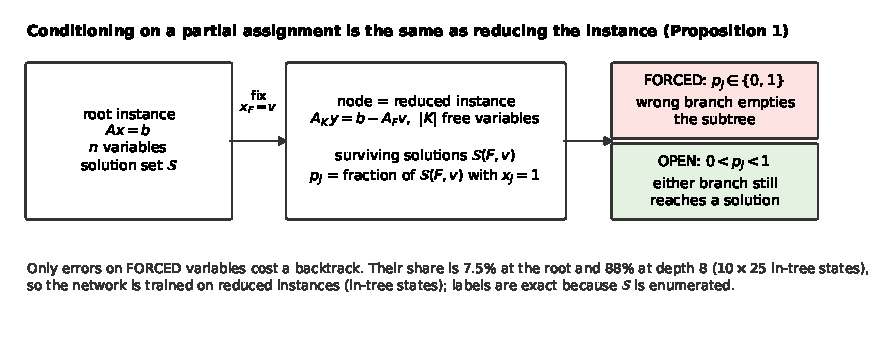
\includegraphics[width=\textwidth]{reduction.pdf}
\caption{Proposition~\ref{prop:reduce} and the partition it induces. A node with $\mathbf{x}_F=\mathbf{v}$ is the smaller BLS $A_K\mathbf{y}=\mathbf{b}-A_F\mathbf{v}$; its conditional marginals are the ordinary marginals of that instance. Variables on which every surviving solution agrees are $\FORCED$; only branching against them costs a backtrack.}
\label{fig:reduction}
\end{figure*}

A node of a depth-first search over~\eqref{eq:bls} is a partial assignment $\mathbf{x}_F=\mathbf{v}$ on a set $F$ of fixed variables, with $K$ the free ones. Let $\SOL(F,\mathbf{v})=\{\mathbf{x}\in\SOL:\mathbf{x}_F=\mathbf{v}\}$ be the solutions consistent with the node and
\begin{equation}
p_j=\Pr[x_j{=}1\mid A,\mathbf{b},\mathbf{x}_F{=}\mathbf{v}]=\frac{|\{\mathbf{x}\in\SOL(F,\mathbf{v}):x_j{=}1\}|}{|\SOL(F,\mathbf{v})|},\quad j\in K,
\label{eq:marginal}
\end{equation}
the conditional marginal, the posterior under the uniform prior on $\SOL$ that a planted-solution generator induces.

\begin{proposition}
\label{prop:reduce}
With $A_F,A_K$ the column submatrices indexed by $F,K$, the map $\mathbf{x}\mapsto\mathbf{x}_K$ is a bijection from $\SOL(F,\mathbf{v})$ onto $\{\mathbf{y}\in\{0,1\}^{|K|}:A_K\mathbf{y}=\mathbf{b}-A_F\mathbf{v}\}$. Hence the conditional marginals of the original instance are the ordinary marginals of the reduced instance.
\end{proposition}
\begin{proof}
$A\mathbf{x}=A_F\mathbf{x}_F+A_K\mathbf{x}_K$; with $\mathbf{x}_F=\mathbf{v}$ fixed, $A\mathbf{x}=\mathbf{b}$ iff $A_K\mathbf{x}_K=\mathbf{b}-A_F\mathbf{v}$, and $\mathbf{x}_F$ is determined, so the map is a bijection; the marginal statement follows by counting.
\end{proof}

Two consequences (Figure~\ref{fig:reduction}). First, one architecture, one label generator and one training loop serve every node: a depth-$d$ training state is stored as an instance on $n-d$ variables, and a network trained on small instances is evaluated on the reduced instances that a search on a larger one produces. Second, $p_j\in\{0,1\}$ means every surviving solution agrees on $x_j$, and branching the other way empties the subtree. We call such variables $\FORCED$ and the rest $\FREE$: either branch of a $\FREE$ variable still reaches a solution, so a wrong first value costs nothing beyond exploring a subtree that contains one. Only $\FORCED$ errors cost a backtrack.

\subsection{What a node looks like, and the accuracy ceiling}
\label{sec:problem-ceiling}

Because $\SOL(F,\mathbf{v})$ can be enumerated on small instances, the Bayes-optimal per-variable accuracy of any predictor of a solution is computable,
\begin{equation}
\mathrm{ceil}(F,\mathbf{v})=\frac{1}{|K|}\sum_{j\in K}\max(p_j,1-p_j),
\label{eq:ceiling}
\end{equation}
attained by answering the majority value of the surviving solutions. Figure~\ref{fig:prediction}a shows how a node changes with depth on $10\times25$ instances: the surviving solution set shrinks from a median of $21$ at the root to a singleton by depth $7$, and the $\FORCED$ share of the free variables rises from $7.5\%$ to $61\%$ at depth $5$, $88\%$ at depth $8$ and $98\%$ at depth $12$. At the root almost no decision can cost anything and the ceiling~\eqref{eq:ceiling} is dominated by $\FREE$ variables; from depth $5$ on, most decisions can. This is the regime a branching heuristic must be good in, and it is where prediction is trained and evaluated below.

\section{Proposed method}
\label{sec:method}

\subsection{Overview}
\label{sec:method-overview}

The solver has two stages (Figure~\ref{fig:framework}). Stage~A is lattice reduction in the Aardal--Hurkens--Lenstra embedding, a sound classical method that returns a verified solution when it succeeds. Stage~B is a depth-first search whose branching decisions are guided by a learned network; nothing learned ever fixes a variable or prunes, so the search stays complete. The network (Figure~\ref{fig:network}) is trained in two stages (Figure~\ref{fig:training}): Stage~1 fits its marginal head to exact conditional marginals of enumerated instances, Stage~2 adds a policy head on the frozen trunk and fine-tunes it on the exact number of nodes that every branching decision costs.

\subsection{Lattice stage}
\label{sec:method-lattice}

The embedding of \citet{aardal2000diophantine} maps~\eqref{eq:bls} to a lattice in $\mathbb{Z}^{n+1+m}$ with basis rows $(2\mathbf{e}_j\mid 0\mid N A_{:,j})$ for $j=1,\dots,n$ and $(\mathbf{1}\mid 1\mid N\mathbf{b})$, with $N$ a large constant. For a solution $\mathbf{x}$, the integer combination with coefficients $(\mathbf{x},-1)$ has constraint part $N(A\mathbf{x}-\mathbf{b})=\mathbf{0}$, indicator $-1$ and variable part in $\{\pm1\}^n$: a vector of squared length $n+1$, among the shortest in the lattice because any vector that violates a row carries a multiple of $N$. We LLL-reduce the basis and then BKZ-reduce it with block size $12$ \citep{lenstra1982factoring,schnorr1994lattice}, scan the reduced basis for rows of that form, decode $x_j=(1-w_jw_{n+1})/2$, verify $A\mathbf{x}=\mathbf{b}$ and return only verified solutions; up to ten random column permutations are tried. The stage costs $0.001$\,s per instance at $n=25$, $0.16$\,s at $n=60$ and $0.54$\,s at $n=80$.

Its coverage falls with size for a reason that is visible in the reduced basis (Figure~\ref{fig:lattice}). Vectors with indicator $0$ and zero constraint part correspond to integer kernel vectors $\mathbf{z}$ with $A\mathbf{z}=\mathbf{0}$; their variable part is $2\mathbf{z}$, so a kernel vector with $k$ nonzero entries has squared length $4k$, and the kernel has rank $n-\operatorname{rank}A\approx 0.65\,n$ on our instances. At $n=25$ the shortest kernel vector in the reduced basis has median squared length $16$ against a solution's $26$, and every basis contains a solution row. At $n=60$ the median shortest kernel vector has squared length $40$ against $61$ and $39$ of the $61$ basis rows are kernel vectors; a solution row survives in $2$ of $30$ bases under one permutation and in $33$--$53\%$ of instances with ten. At $n\ge70$ the shortest kernel vectors are shorter than the solution by $13$--$19$ units and a solution row never appears. Reduction fills the basis with the shortest vectors it can find, and from $n\approx60$ those are kernel vectors, not solutions. This is why the learned search, not the lattice, carries the sizes we care about.

\begin{figure}[t]
\centering
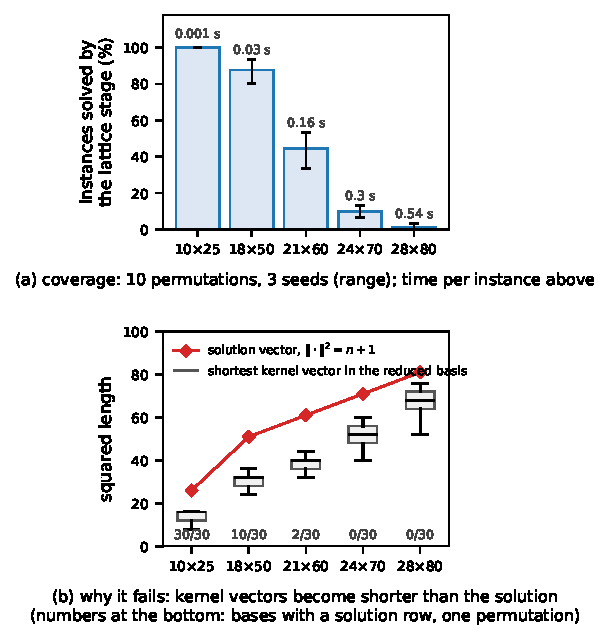
\includegraphics[width=\columnwidth]{lattice.pdf}
\caption{The lattice stage. (a) Fraction of instances it solves with ten column permutations, three seeds (bars: mean, whiskers: range; number above: median time per instance). (b) Squared length of the shortest kernel-type vector in the reduced basis (boxes over $30$ instances, one permutation) against the squared length $n+1$ of a solution vector; the numbers at the top count the instances whose reduced basis contains a solution row.}
\label{fig:lattice}
\end{figure}

\subsection{Guided depth-first search}
\label{sec:method-search}

Every instance the lattice stage does not close is searched from scratch by the depth-first procedure of Algorithm~\ref{alg:node}. A node is a partial assignment; by Proposition~\ref{prop:reduce} it is handled as the reduced instance $(A',\mathbf{b}')=(A_K,\mathbf{b}-A_F\mathbf{v})$, and $r_i$ denotes the number of free variables in row $i$ of $A'$.

\begin{table}[t]
\centering
\caption{Algorithm 1: one node of the guided depth-first search. Steps 1--4 are sound and are the only steps that fix variables or prune; the learned components enter only at step 5.}
\label{alg:node}
\fitc{\begin{tabular}{@{}rp{0.9\columnwidth}@{}}
\toprule
1 & \textbf{Reduce.} Pop $(F,\mathbf{v})$; form $A'=A_K$, $\mathbf{b}'=\mathbf{b}-A_F\mathbf{v}$. Drop rows with $r_i=0$; if none remain, verify $A\mathbf{x}=\mathbf{b}$ and return $\mathbf{x}$. \\
2 & \textbf{Bound check.} If $b'_i<0$ or $b'_i>r_i$ for some row, discard the node. \\
3 & \textbf{Propagate.} While some row has $b'_i=0$ (fix its free variables to $0$) or $b'_i=r_i$ (fix them to $1$): apply the fixings; on a contradiction discard the node; if variables were fixed, push the reduced node and return. \\
4 & \textbf{Relax.} Re-optimise the single warm-started relaxation $\{A\mathbf{x}=\mathbf{b},\ 0\le\mathbf{x}\le1\}$ with the bounds of $F$ tightened to $\mathbf{v}$ (dual simplex from the previous basis, $0.08$\,ms). If infeasible, discard the node; else read the vertex $\mathbf{x}^{LP}_K$. \\
5 & \textbf{Predict.} One forward pass of the network on the bipartite graph of $(A',\mathbf{b}',\mathbf{x}^{LP}_K)$ gives $\hat p_j$ and $g_j$ for $j\in K$ ($1.9$\,ms at a $21\times60$ root). Choose $j^\star=\arg\max_j g_j$ and $v=\mathbb{1}[\hat p_{j^\star}\ge\frac12]$. \\
6 & \textbf{Branch.} Push the child $x_{j^\star}=1-v$, then the child $x_{j^\star}=v$, so that $v$ is explored first and $1-v$ on backtracking. \\
\bottomrule
\end{tabular}}
\end{table}

Three design choices matter for what follows. Propagation on a $0/1$ row reads ``exactly $b'_i$ of the $r_i$ free variables in this row are $1$'' and can fix variables only when $b'_i\in\{0,r_i\}$, which is why it is inert near the root of our instances. The relaxation is not rebuilt per node: one linear program over the original $n$ variables is kept for the whole search and a node is expressed as a set of bound changes, so consecutive nodes, a child or a sibling after backtracking, differ by a few bounds and the dual simplex resumes from the parent basis; this is $50\times$ cheaper than rebuilding and is what lets the loop process about $700$ nodes per second in Python. Its infeasibility test is strictly stronger than propagation, since it sees linear combinations of rows, and it is the last sound step before the network. The vertex $\mathbf{x}^{LP}$ it returns is the main input feature of the network.

\subsection{Stage 1: exact conditional marginals as the target}
\label{sec:method-stage1}

\begin{figure*}[t]
\centering
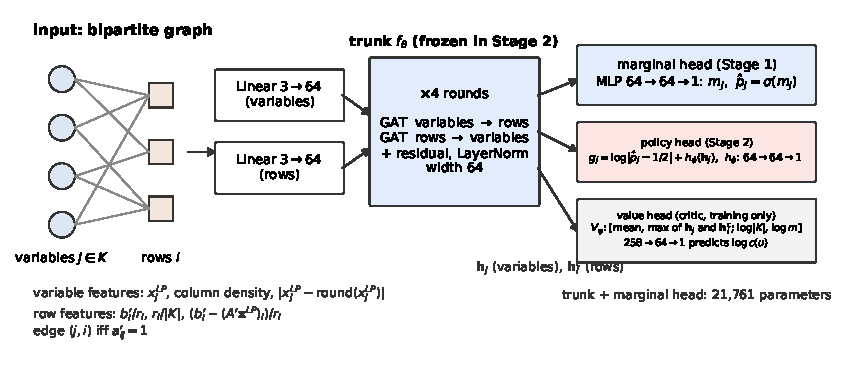
\includegraphics[width=\textwidth]{network.pdf}
\caption{The network. The reduced instance enters as a bipartite graph with three features per variable and per row; a trunk of four graph-attention rounds produces an embedding per variable and per row; three heads read them. The marginal head is trained in Stage~1, the policy head in Stage~2 on the frozen trunk, and the value head serves only as the critic during Stage~2.}
\label{fig:network}
\end{figure*}

\begin{figure*}[t]
\centering
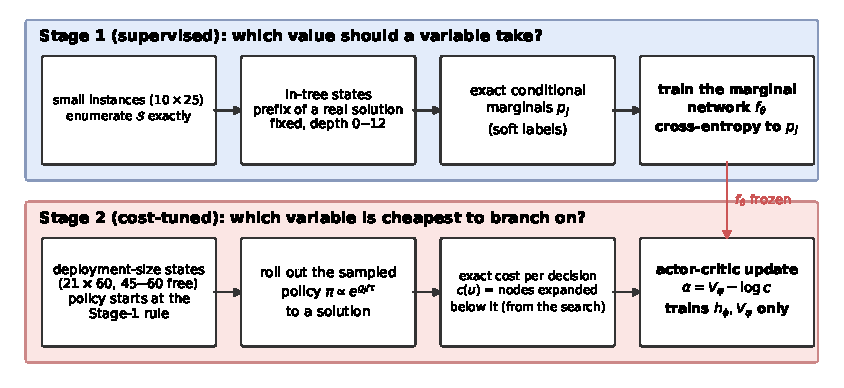
\includegraphics[width=\textwidth]{training.pdf}
\caption{The two training stages. Stage~1 learns \emph{which value} from exact conditional marginals of enumerable instances; Stage~2 learns \emph{which variable} from the exact number of nodes every decision costs, produced by the search, with the Stage-1 network frozen.}
\label{fig:training}
\end{figure*}

\paragraph{Network.} The network $f_\theta$ (Figure~\ref{fig:network}) is a bipartite variable--constraint graph network with graph attention \citep{velickovic2018graph}, the architecture family of \citet{gasse2019exact}. Each variable node carries three features (its relaxation value $x^{LP}_j$, its column density, its fractionality $|x^{LP}_j-\mathrm{round}(x^{LP}_j)|$), each constraint node three (its right-hand side $b'_i/r_i$, its density $r_i/|K|$, its relaxation residual $(b'_i-(A'\mathbf{x}^{LP})_i)/r_i$), and an edge joins $j$ to $i$ where $a'_{ij}=1$. Linear layers lift both to width $64$; four rounds of attention then alternate variable-to-constraint and constraint-to-variable messages with residual connections and layer normalisation, and a two-layer marginal head maps each variable embedding $\mathbf{h}_j$ to one logit, $\hat p_j=\sigma(m_j)$; $21{,}761$ parameters in all. The two heads added in Stage~2 are described in Section~\ref{sec:method-stage2}. The architecture is standard; the contribution is the target.

\paragraph{Target and training states.} On instances small enough to enumerate ($10\times25$), $\SOL$ is obtained with the all-solutions mode of a constraint solver and $p_j$ computed by counting. Only enumerations that run to exhaustion are accepted; a time-limited enumeration with solutions already collected would substitute a truncated $\SOL$ and bias every label. Training states are reachable in-tree states: a depth $d\in\{0,\dots,12\}$ is drawn uniformly, a prefix of an LP-confidence variable ordering is fixed to the values of a randomly chosen actual solution, and the reduced instance is enumerated in turn to give $p_j$ on its free variables. The network is trained by cross-entropy against the soft targets,
\begin{equation}
\mathcal{L}_1=-\tfrac{1}{|K|}\sum_{j\in K}\bigl[p_j\log\hat p_j+(1-p_j)\log(1-\hat p_j)\bigr],
\label{eq:loss1}
\end{equation}
which is minimised exactly at $\hat p=p$; replacing $p_j$ by the planted solution, the usual choice, is a noisy surrogate whenever $|\SOL|>1$.

\paragraph{Branching rule.} At a node the network is evaluated once and the Stage-1 rule branches on the most confident marginal with its majority value,
\begin{equation}
j^\star=\arg\max_{j\in K}\,|\hat p_j-\tfrac12|,\qquad v=\mathbb{1}[\hat p_{j^\star}\ge\tfrac12].
\label{eq:rule1}
\end{equation}

\subsection{Stage 2: exact subtree node counts as the objective}
\label{sec:method-stage2}

Rule~\eqref{eq:rule1} maximises the chance that the first child contains a solution. It says nothing about how much the search pays when it does not, nor how much smaller the children become; both are properties of the subtree, and a depth-first search produces them exactly. For a node $u$ let $c(u)$ be the number of nodes expanded below $u$ until a solution is found there or the subtree is exhausted; the search returns it when it backtracks out of $u$. We use $c(u)$ as the cost of the branching decision made at $u$; $c(\text{root})$ is the number of nodes the whole search expands to reach a solution, which is the tree-size metric reported throughout the experiments. Stage~2 fine-tunes the branching order on $-\log c(u)$.

\paragraph{Decision process.} A state is the reduced instance after propagation; an action is a free variable $j$; the first value stays $\mathbb{1}[\hat p_j\ge\frac12]$ from the frozen Stage-1 network. Because each decision owns its subtree, credit is assigned per decision rather than per episode, the property a sparse solved/unsolved reward lacks and the one that makes the problem well posed \citep{etheve2020reinforcement}.

\paragraph{Policy and value heads.} On the frozen trunk of $f_\theta$ two heads are added (Figure~\ref{fig:network}). The policy logit is
\begin{equation}
g_j(s)=\log\bigl|\hat p_j-\tfrac12\bigr|+h_\phi(\mathbf{h}_j),
\label{eq:policy}
\end{equation}
with $h_\phi$ a two-layer network whose last layer is initialised to zero, so that $\pi(j\mid s)\propto\exp(g_j/\tau)$ starts as a softening of rule~\eqref{eq:rule1} and its argmax is exactly that rule. A value head $V_\psi(s)$ on the mean- and max-pooled variable and constraint embeddings, $\log|K|$ and $\log m$ predicts $\log c$.

\paragraph{Update.} Each epoch samples $400$ training states with $45$--$60$ free variables, rolls the sampled policy ($\tau=1$) out to a solution, and records every decision with its exact cost, about $21{,}000$ decisions per epoch. With the advantage $\alpha(u)=V_\psi(s_u)-\log c(u)$ standardised within the epoch,
\begin{equation}
\begin{split}
\mathcal{L}_2=\sum_u\Bigl[&-\alpha(u)\log\pi(j_u\mid s_u)-\lambda\,\mathcal{H}\bigl(\pi(\cdot\mid s_u)\bigr)\\
&+\bigl(V_\psi(s_u)-\log c(u)\bigr)^2\Bigr],\qquad\lambda=0.01,
\end{split}
\label{eq:loss2}
\end{equation}
an on-policy actor-critic update with Monte-Carlo returns \citep{williams1992simple}; no bootstrapping is needed because the return is exact. Only $\phi,\psi$ are trained; $\theta$ is fixed, so the marginal that chooses values and defines the $\FORCED$/$\FREE$ partition is unchanged, and any improvement is attributable to the branching order alone. The critic is pre-trained on decisions recorded under rule~\eqref{eq:rule1}, and its held-out rank correlation with $\log c$ gates the actor update, since a baseline that cannot rank costs turns the advantage into noise. The epoch is selected by the total node count below held-out states of the training pool, never on evaluation instances. At deployment the policy is greedy, $j^\star=\arg\max_j g_j(s)$.

\subsection{Cost per node}
\label{sec:method-cost}

At a node with $|K|$ free variables the guided search pays one warm-started relaxation and one forward pass; the forward pass is over $90\%$ of the node cost at $21\times60$. The sound procedure that detects the same $\FORCED$ variables, LP-probing (fix $x_j$ to each value and prune the one that makes the relaxation infeasible), pays $|K|$ relaxations; with warm starts on both sides the measured ratio grows from $1.7\times$ at $n=25$ to $7.2\times$ at $n=60$. The Stage-2 heads add nothing measurable.

\section{Experiments}
\label{sec:exp}

The experiments answer four questions: does learned branching beat classical branching in the same search (Section~\ref{sec:res-branching}); does it transfer to sizes it was not trained at (Section~\ref{sec:res-transfer}); how far is it from a complete solver (Section~\ref{sec:res-solvers}); and is every component necessary (Section~\ref{sec:res-ablation}).

\subsection{Setup}
\label{sec:exp-setup}

\paragraph{Instances.} Instances are generated as in Section~\ref{sec:problem-instances}, the market-split construction with $0/1$ coefficients and a planted solution. Sizes are $10\times25$, $18\times50$, $21\times60$, $24\times70$ and $28\times80$; $m$ is chosen per size so that the median number of solutions is comparable where it can be verified by enumeration ($|\SOL|$: $23$, $19$ and $10$ at $n=25$, $50$, $60$; $27/30$ verified at $60$) and by constraint density $m/n\approx0.35$ at $n\ge70$, where enumeration does not complete. At $n=100$ CP-SAT finds no solution within $20$\,s and every strategy fails, so $n=80$ is the last size. Evaluation uses $30$ instances per size and a $100$-instance $21\times60$ set (generator seeds $700000$--$700099$, which contains the thirty); Stage~1 trains on $10{,}000$ in-tree states from $1{,}760$ separate $10\times25$ instances, Stage~2 on a separate $21\times60$ pool of $500$ instances (seeds $800000$+, $400/100$ split) whose $100$ held-out instances supply the epoch-selection states. Overlap between any training pool and any evaluation set is zero by hash of $(A,\mathbf{b})$.

\paragraph{Training.} Stage~1: Adam, learning rate $10^{-3}$, $20$ epochs, batch $1$, gradient clipping $1.0$; $20$ minutes on one CPU core; no hyperparameter was tuned and there is no validation split. Stage~2: critic pre-training on $37{,}275$ recorded decisions ($9{,}375$ held-out), then six epochs of the update~\eqref{eq:loss2}; two training seeds. The policy fine-tuned at $21\times60$ is denoted Stage~1+2\,(60); a second policy fine-tuned at $18\times50$ with the same protocol, Stage~1+2\,(50), tests upward transfer.

\begin{table}[t]
\centering
\caption{Branching arms. All run in the same depth-first loop (Algorithm~\ref{alg:node}: one warm-started relaxation per node, the same propagation, the same budget) and differ only in step 5; the number in parentheses is the size the learned component was trained at. The LP rule is not a solver: it is the same loop with the relaxation vertex in place of the network.}
\label{tab:arms}
\fitc{\begin{tabular}{lll}
\toprule
arm & branches on & first value \\
\midrule
random & a random free variable & random \\
LP rule & most integral relaxation value, $\arg\max_j|x^{LP}_j-\tfrac12|$ & $\mathrm{round}(x^{LP}_j)$ \\
Stage 1 (25) & most confident marginal, $\arg\max_j|\hat p_j-\tfrac12|$ & $\mathbb{1}[\hat p_j\ge\tfrac12]$ \\
Stage 1+2 (60 / 50) & cost-tuned score, $\arg\max_j g_j$ & $\mathbb{1}[\hat p_j\ge\tfrac12]$ \\
\bottomrule
\end{tabular}}
\end{table}

\paragraph{Arms and solvers.} Table~\ref{tab:arms} defines the branching arms. The random arm checks that the instances are hard; the LP rule is the classical most-integral rule and the reference for branching quality. CP-SAT (OR-Tools) and SCIP are run as complete solvers on the same instances, single-threaded, under the same budgets, as the wall-clock reference.

\paragraph{Protocol and metrics.} Two metrics are reported per instance: the number of nodes the search expands to reach a solution, $c(\text{root})$ of Section~\ref{sec:method-stage2}, which measures branching quality and is seed-invariant because the search is deterministic given the relaxation vertex; and wall-clock time, which also reflects the cost per node. Budgets are per-instance wall-clock ($60$, $300$, $600$, $1{,}200$, $1{,}200$\,s for the five sizes), enforced by process termination; six instances run concurrently on a $20$-core machine and all timing-sensitive code is single-threaded (no GPU is used). Per-instance speed is compared with a two-sided sign test. Every $21\times60$ figure is replicated over three evaluation seeds, and the lattice stage is switched off for the branching comparisons and on for the cascade (Section~\ref{sec:res-cascade}). Enumeration and CP-SAT use OR-Tools; lattice reduction uses fpylll; the relaxation uses Gurobi's dual simplex.

\subsection{Learned branching against classical branching}
\label{sec:res-branching}

\begin{table}[t]
\centering
\caption{Branching strategies in the same warm-started loop, lattice stage off, three seeds (mean $\pm$ s.d.\ of per-seed medians; node counts are seed-invariant). Stage~1+2 is the policy fine-tuned at $21\times60$, reported for two training seeds.}
\label{tab:search}
\fitc{\begin{tabular}{llrrr}
\toprule
size (budget) & strategy & solved & median nodes & median time \\
\midrule
$10\times25$ (60\,s) & LP rule & 30/30 & 46 & $0.03$\,s \\
 & Stage 1 & 30/30 & 24 & $0.07$\,s \\
\midrule
$18\times50$ (300\,s) & LP rule & 30/30 & 4{,}224 & $2.43\pm0.33$\,s \\
 & Stage 1 & 30/30 & 1{,}085 & $1.82\pm0.37$\,s \\
 & Stage 1+2 & 30/30 & \textbf{424} & $\mathbf{0.52\pm0.01}$\,\textbf{s} \\
\midrule
$21\times60$, 100 inst.\ (600\,s) & LP rule & 100/100 & 79{,}609 & $41.2\pm1.9$\,s \\
 & Stage 1 & 100/100 & 13{,}386 & $16.5\pm0.6$\,s \\
 & Stage 1+2 (seed 0 / 1) & 100/100 & 5{,}495 / \textbf{4{,}940} & $7.6$ / $\mathbf{6.8}$\,s \\
\bottomrule
\end{tabular}}
\end{table}

Table~\ref{tab:search} and Figure~\ref{fig:results}b give the main result. Stage~1 produces a smaller tree than the LP rule at every size, by $2.0\times$, $3.9\times$ and $5.5\times$ nodes, and the ratio grows with size. A smaller tree buys time only once the tree is large enough to pay for the forward pass: at $10\times25$ Stage~1 is slower, from $18\times50$ it is faster ($1.3$--$1.4\times$, not significant on $30$ instances), and on the $100$-instance $21\times60$ set it is $2.0$--$2.3\times$ faster on $70$--$71$ of $100$ instances ($p<0.001$). Stage~2 removes a further $2.3$--$2.4\times$ of the nodes and $2.0$--$2.4\times$ of the time ($64$--$68/100$, $p\le0.007$) at unchanged per-node cost, in both training seeds and every evaluation seed, for $4.8$--$5.9\times$ over the LP rule end to end; the fine-tuned policy also transfers down to $18\times50$ ($2.6\times$ fewer nodes, $1.8$--$2.2\times$ faster, $p\le0.016$). Random branching solves none of $30$ instances at $20\times50$ within $300$\,s and none of the $21\times60$ residual of Section~\ref{sec:res-cascade}: the instances are hard, and every sound arm closes all of them, so the comparison is about nodes and time.

\begin{figure*}[t]
\centering
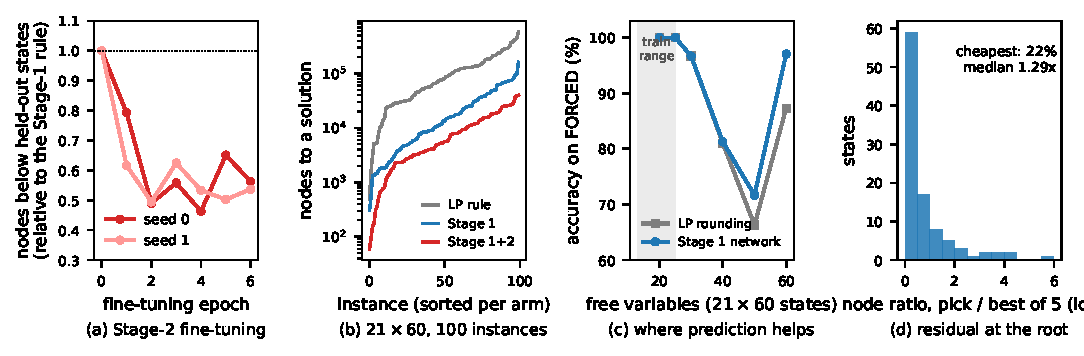
\includegraphics[width=\textwidth]{results.pdf}
\caption{(a) Stage-2 fine-tuning: nodes expanded below $150$ held-out states relative to the Stage-1 rule, two training seeds; the selected epochs are $4$ and $2$. (b) Nodes to a solution on the $100$-instance $21\times60$ set, each arm sorted. (c) Accuracy on $\FORCED$ variables of $21\times60$ in-tree states by number of free variables: the Stage-1 margin over relaxation rounding lies outside its training range. (d) Residual at the root: nodes below the confidence rule's choice relative to the cheapest of its five candidates ($100$ held-out states, $45$--$50$ free variables).}
\label{fig:results}
\end{figure*}

\subsection{Transfer across sizes}
\label{sec:res-transfer}

\begin{table}[t]
\centering
\caption{Instances solved within budget by size, lattice off; $30$ instances per size ($100$ at $21\times60$), ranges over three seeds where they differ, $28\times80$ one seed. Training sizes in parentheses.}
\label{tab:solved}
\fitc{\begin{tabular}{lrrrr}
\toprule
size (budget) & LP rule & Stage 1 (25) & Stage 1+2 (60) & Stage 1+2 (50) \\
\midrule
$18\times50$ (300\,s) & 30/30 & 30/30 & 30/30 & 30/30 \\
$21\times60$, 100 inst.\ (600\,s) & 100/100 & 100/100 & 100/100 & 100/100 \\
$24\times70$ (1200\,s) & 23--25/30 & 29/30 & \textbf{30/30} & \textbf{30/30} \\
$28\times80$ (1200\,s) & 4/30 & 8/30 & \textbf{18/30} & 17/30 \\
\bottomrule
\end{tabular}}
\end{table}

\begin{table}[t]
\centering
\caption{Median nodes to a solution by size, lattice off (seed-invariant; same instances as Table~\ref{tab:solved}, medians over solved instances at $28\times80$).}
\label{tab:nodes}
\fitc{\begin{tabular}{lrrrr}
\toprule
size & LP rule & Stage 1 (25) & Stage 1+2 (60) & Stage 1+2 (50) \\
\midrule
$18\times50$ & 4{,}224 & 1{,}085 & \textbf{424} & 1{,}147 \\
$21\times60$, 100 inst. & 79{,}609 & 13{,}386 & \textbf{5{,}495} & 7{,}796 \\
$24\times70$ & 980{,}743 & 260{,}114 & \textbf{90{,}054} & 95{,}818 \\
$28\times80$ & 1{,}929{,}041 & 803{,}535 & \textbf{470{,}606} & 560{,}077 \\
\bottomrule
\end{tabular}}
\end{table}

\begin{table}[t]
\centering
\caption{The same results read by transfer direction: ratio of median nodes, range of per-instance median time ratios over seeds, and the number of instances on which the transferred arm is faster.}
\label{tab:transferdir}
\fitc{\begin{tabular}{llrrr}
\toprule
trained $\to$ tested & vs. & nodes & time & wins \\
\midrule
Stage 1: $25\to50$ & LP rule & $3.9\times$ & $1.3$--$1.4\times$ & 18/30 \\
Stage 1: $25\to60$ & LP rule & $5.5\times$ & $2.0$--$2.3\times$ & 70--71/100 \\
Stage 1: $25\to70$ & LP rule & $3.8\times$ & $0.7$--$1.1\times$ & 16--17/30 \\
Stage 1+2: $60\to50$ (down) & Stage 1 & $2.6\times$ & $1.8$--$2.2\times$ & 22--24/30 \\
Stage 1+2: $50\to60$ (up) & Stage 1 & $2.0\times$ & $1.7$--$1.9\times$ & 63--66/100 \\
Stage 1+2: $60\to70$ (up) & Stage 1 & $2.7\times$ & $2.3$--$3.3\times$ & 22--23/30 \\
Stage 1+2: $50\to70$ (up) & Stage 1 & $2.2\times$ & $2.1$--$2.7\times$ & 19--21/30 \\
Stage 1+2: $50\to50$ (same) & Stage 1 & $0.9\times$ & $1.1$--$1.4\times$ & 16--18/30 \\
\bottomrule
\end{tabular}}
\end{table}

\begin{figure*}[t]
\centering
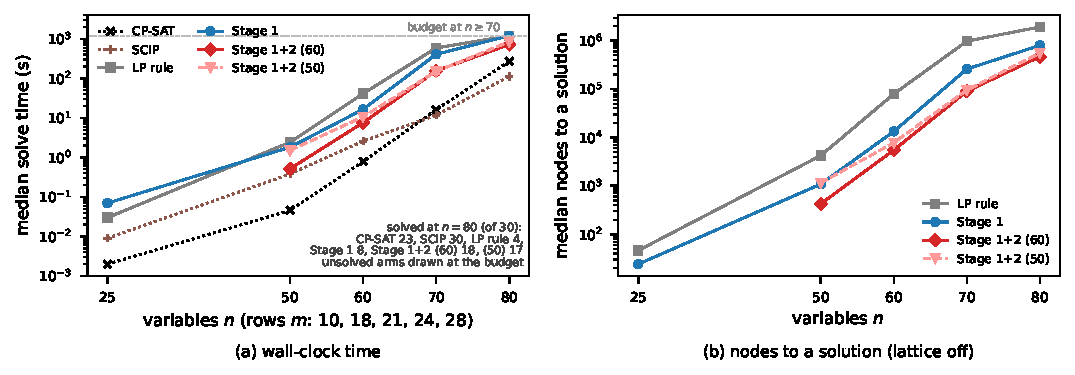
\includegraphics[width=\textwidth]{scaling.pdf}
\caption{Scaling with size. (a) Median wall-clock time of the branching arms and of the complete solvers; at $n\ge70$ whiskers span the three seeds, and unsolved arms at $n=80$ are drawn at the budget with their solve counts in the panel. (b) Median nodes to a solution, lattice off. Both stages were trained at $n\le60$.}
\label{fig:scaling}
\end{figure*}

Both stages transfer in both directions (Tables~\ref{tab:solved}--\ref{tab:transferdir}, Figure~\ref{fig:scaling}). Stage~1, trained only at $10\times25$, keeps a node advantage over the LP rule at every size ($3.9\times$, $5.5\times$, $3.8\times$, $2.4\times$ at $n=50$, $60$, $70$, $80$), but its time advantage shrinks as the tree grows: at $24\times70$ it solves $29/30$ against the LP rule's $23$--$25/30$, yet on the instances both solve it is no faster ($0.7$--$1.1\times$), because a $260{,}000$-node tree pays for $260{,}000$ forward passes. Stage~2 restores the advantage and carries it upward. The policy fine-tuned at $18\times50$ is $2.0\times$ better than Stage~1 in nodes at $21\times60$ ($63$--$66/100$ faster, $p<0.001$); both fine-tuned policies solve $30/30$ at $24\times70$ in every seed, $2.3$--$3.3\times$ and $2.1$--$2.7\times$ faster than Stage~1, at $1.2$--$1.4\times$ their training size; at $28\times80$ they solve $18$ and $17$ of $30$ within $1{,}200$\,s where Stage~1 solves $8$ and the LP rule $4$. That is where the window closes for the learned search: SCIP solves $30/30$ there at a median of $112$\,s.

\subsection{Distance to complete solvers}
\label{sec:res-solvers}

\begin{table}[t]
\centering
\caption{Median wall-clock time by size, single-threaded, same instances and budgets; where an arm does not solve every instance its solve count is in Table~\ref{tab:solved} (CP-SAT $23/30$ at $28\times80$).}
\label{tab:classical}
\fitc{\begin{tabular}{lrrrrrr}
\toprule
size & CP-SAT & SCIP & LP rule & Stage 1 & Stage 1+2 (60) & Stage 1+2 (50) \\
\midrule
$10\times25$ & \textbf{0.002\,s} & 0.009\,s & 0.03\,s & 0.07\,s & --- & --- \\
$18\times50$ & \textbf{0.05\,s} & 0.39\,s & 2.4\,s & 1.8\,s & 0.5\,s & 1.5\,s \\
$21\times60$, 100 inst. & \textbf{0.8\,s} & 2.6\,s & 41\,s & 16.5\,s & 7.6\,s & 10.7\,s \\
$24\times70$ & 16\,s & \textbf{12\,s} & 537--644\,s & 358--457\,s & 125--185\,s & 135--165\,s \\
$28\times80$ & 270\,s & \textbf{112\,s} & $>$1200\,s & $>$1200\,s & 720\,s & 852\,s \\
\bottomrule
\end{tabular}}
\end{table}

\begin{table}[t]
\centering
\caption{Decomposition of the gap to CP-SAT at $21\times60$ ($30$ instances). CP-SAT's branch counter and our node counter are not the same unit (branches include restarts and exclude what clause learning skips), so the first row is a comparison of magnitude only.}
\label{tab:throughput}
\fitc{\begin{tabular}{lrr}
\toprule
& CP-SAT & Stage 1+2 \\
\midrule
branches / nodes to a solution (median) & 18{,}827 & 4{,}040--8{,}873 \\
branches / nodes per second & 19{,}782 & $\approx700$ \\
median time & 1.16\,s & 5.9--12.5\,s \\
\bottomrule
\end{tabular}}
\end{table}

Table~\ref{tab:classical} places the learned search next to the complete solvers on the same instances. CP-SAT is $9$--$11\times$ faster than the full method at $18\times50$ and $21\times60$, and from $24\times70$ SCIP is the fastest, $10$--$15\times$ ahead. Table~\ref{tab:throughput} decomposes the gap: CP-SAT does not search a smaller tree than we do, it processes each node about $28\times$ faster, in C++ with clause learning and restarts, where our loop runs in Python and spends over $90\%$ of each node in the network's forward pass. The deficit is per-node throughput, not branching quality; whether a compiled inference path and clause learning close it is not shown here.

\subsection{Ablations}
\label{sec:res-ablation}

\subsubsection{The Stage-1 signal: in-tree labels, then graph structure}
\label{sec:res-stage1}

\begin{figure*}[t]
\centering
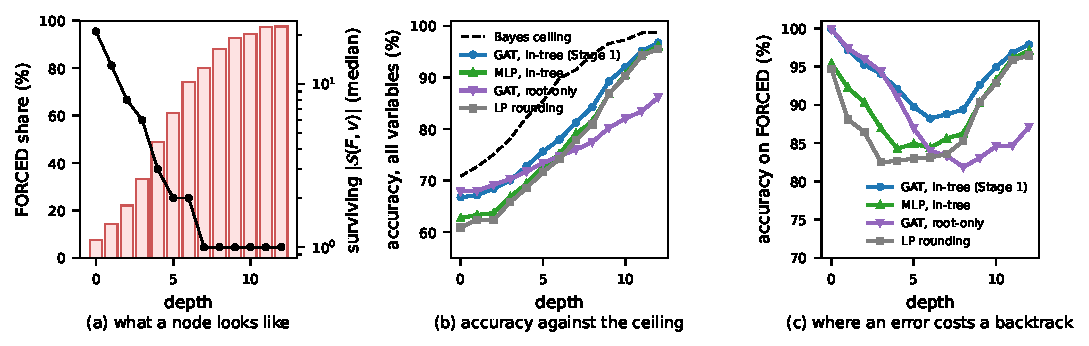
\includegraphics[width=\textwidth]{prediction.pdf}
\caption{Prediction against the exact posterior on $2{,}640$ held-out in-tree states of $10\times25$ instances, by depth. (a) The $\FORCED$ share of free variables and the median number of surviving solutions. (b) Per-variable accuracy on all free variables against the Bayes ceiling~\eqref{eq:ceiling}. (c) Accuracy on $\FORCED$ variables, where an error costs a backtrack. Four predictors share the labels, the loss and the states: the Stage-1 network (a GAT trained in-tree), the same GAT trained on root states only, a graph-free MLP with constraint aggregates trained in-tree, and relaxation rounding.}
\label{fig:prediction}
\end{figure*}

\begin{table}[t]
\centering
\caption{Accuracy on $\FORCED$ variables of held-out in-tree states of $10\times25$ instances, where an error costs a backtrack; ground truth is the reference solution, and the ceiling is $100\%$ by definition. Accuracy on all free variables is in Figure~\ref{fig:prediction}b.}
\label{tab:pred}
\fitc{\begin{tabular}{lrr}
\toprule
predictor & all depths & depth 8 \\
\midrule
GAT, in-tree (Stage 1) & \textbf{93.2\%} & \textbf{89.4\%} \\
MLP, in-tree & 89.5\% & 86.2\% \\
GAT, root-only (control) & 88.0\% & 81.9\% \\
LP rounding & 87.9\% & 85.3\% \\
\midrule
$\FORCED$ share of variables & 57.2\% & 87.9\% \\
\bottomrule
\end{tabular}}
\end{table}

Table~\ref{tab:pred} and Figure~\ref{fig:prediction} isolate what makes the Stage-1 signal work. The in-tree labels come first. A network with the same architecture, labels, optimiser and number of states, trained on root states only, is better than the in-tree network at the root ($67.9\%$ against $66.7\%$ on all free variables) and worse from depth $4$ on; over all depths it is below relaxation rounding on every variable ($75.5\%$ against $76.5\%$) and, on the $\FORCED$ variables at depth $8$, $3.4$ points below it. Root-level accuracy is the wrong objective for a branching heuristic because almost nothing at the root can cost anything. The graph structure comes second. A graph-free MLP on the same per-variable features plus mean and max aggregates of its incident rows, trained on the same in-tree states, reaches $89.5\%$ on $\FORCED$ variables against the GAT's $93.2\%$; on a matched $2{,}000/800$ split its $L_1$ distance to the exact marginal is $0.225$ against $0.151$. The label effect ($5$--$7$ points on $\FORCED$ variables) is larger than the structure effect ($3$--$4$ points), and both are needed to stay above the classical rule at every depth. Within the training size, the depth range of the training states does not matter (depths $0$--$6$, $6$--$12$ and $0$--$12$ give $79.3$, $79.9$ and $79.9\%$).

Where the margin lives at deployment size is shown in Figure~\ref{fig:results}c on $21\times60$ in-tree states: inside the training range ($13$--$25$ free variables) the network and rounding are indistinguishable, because at constraint density $m/|K|\ge0.8$ the relaxation is already integral on every $\FORCED$ variable; the entire margin ($+5$ points) arises at $50$--$60$ free variables, outside the training range, where the relaxation is weakest. $80\%$ of the queries a $21\times60$ search makes fall there.

\subsubsection{The two signals are not interchangeable}
\label{sec:res-signals}

\begin{figure*}[t]
\centering
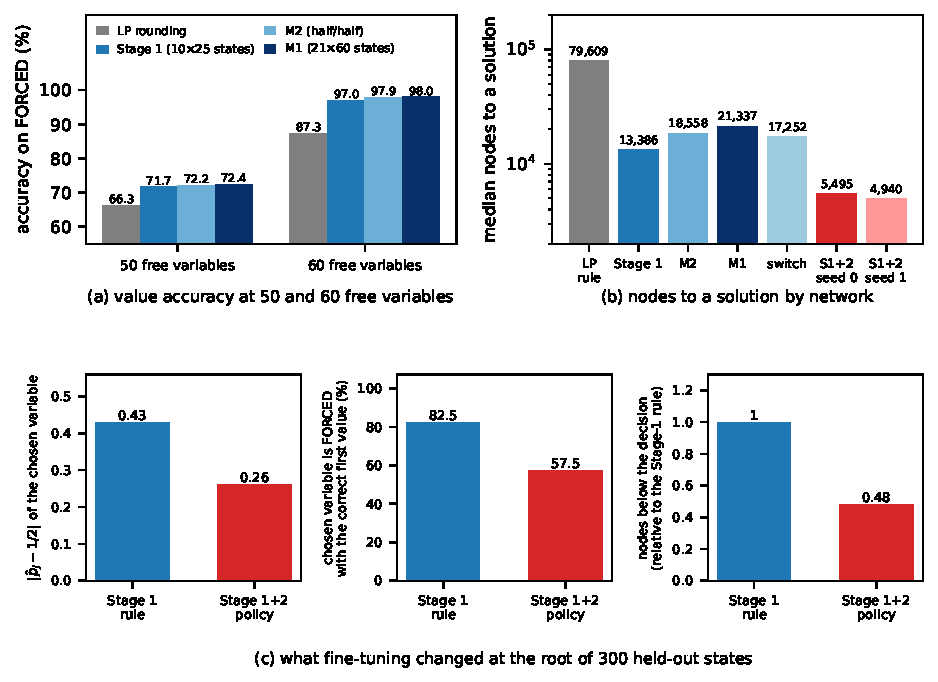
\includegraphics[width=\textwidth]{signals.pdf}
\caption{Value accuracy and tree size move independently. (a) Accuracy on $\FORCED$ variables of $21\times60$ in-tree states with $50$ and $60$ free variables, for relaxation rounding, the Stage-1 network trained on $10\times25$ states, and the same architecture trained on $21\times60$ states (M1) or on a half-and-half mix (M2). (b) Median nodes to a solution on the $100$-instance set: the networks with the higher value accuracy expand more nodes; the cost-tuned policy expands fewer. (c) At the root of $300$ held-out states the fine-tuned policy picks a less confident variable that is less often $\FORCED$-and-correct, and the number of nodes below its decision is half.}
\label{fig:signals}
\end{figure*}

\paragraph{Sharpening the value signal enlarges the tree.} Figure~\ref{fig:results}c suggests an obvious fix: train Stage~1 where its margin lives. We built $2{,}691$ in-tree states with $30$--$60$ free variables from the $21\times60$ training pool (exact marginals; every state with at most $55$ free variables enumerates within $90$\,s) and trained the same architecture on them alone (M1) and on a half-and-half mix with the $10\times25$ states (M2). Accuracy on $\FORCED$ variables at $50$ and $60$ free variables rises by about one point ($71.7\to72.4\%$ and $97.0\to98.0\%$, Figure~\ref{fig:signals}a). The tree grows: M1 expands a median of $21{,}337$ nodes on the $100$-instance set against $13{,}386$ for Stage~1 (fewer on only $38/100$, $p=0.021$), M2 $18{,}558$, and a switch that routes nodes with at least $50$ free variables to M1 and the rest to Stage~1 recovers nothing ($17{,}252$; Figure~\ref{fig:signals}b). The reason is where the decisions are: two thirds of them occur at $25$--$34$ free variables, and on such small dense states M1's most confident variable is $\FORCED$-and-correct $77.6\%$ of the time against $94.4\%$ for Stage~1 (rank correlation with the true margin $0.12$ against $0.36$). A network slightly better at the top of the tree and much worse inside it makes the search slower; the training distribution of the value signal is not the lever.

\paragraph{The confident choice is rarely the cheapest.} On $100$ held-out states with $45$--$50$ free variables we forced the root to each of the five most confident variables and ran rule~\eqref{eq:rule1} below (Figure~\ref{fig:results}d). The rule's own choice is the cheapest of the five on $22\%$ of states; the median ratio of its node count to the best candidate's is $1.29$, the mean $2.97$, a candidate at least twice as cheap exists on $24\%$ of states, and the best root choice alone would remove $55\%$ of the nodes summed over these states. The residual is about \emph{which} variable, and it is large.

\paragraph{The cost signal moves away from confidence.} The critic on the frozen trunk reaches a held-out Spearman correlation of $0.80$ with $\log c$ (a baseline that knows only the state's size: $0.70$; within the $35$--$44$ free-variable bucket $0.68$ against $0.38$); unfreezing the trunk adds $0.02$ and is not used. Six fine-tuning epochs bring the number of nodes below held-out states to $0.46$ (seed $0$, epoch $4$ selected) and $0.50$ (seed $1$, epoch $2$) of the Stage-1 rule's, with the policy entropy falling from $1.7$ to below $0.1$ (Figure~\ref{fig:results}a). On $300$ held-out states the fine-tuned policy branches on a different root variable than rule~\eqref{eq:rule1} at $95\%$ of them; its pick is typically the $15$th most confident ($|\hat p-\frac12|$ of $0.26$ against $0.43$) and is $\FORCED$ with a correct first value less often ($57.5\%$ against $82.5\%$; Figure~\ref{fig:signals}c). By the value criterion the fine-tuned choice is worse on every count, and the tree is less than half the size. The gain is not a property of the root decision alone: forcing only the root to the fine-tuned pick with rule~\eqref{eq:rule1} below gives a median node ratio of $0.93$ (cheaper on $22/46$), so it is the sequence of decisions that improves. Two training seeds reach similar node counts while choosing different variables at many nodes, as expected if the objective, not a particular solution, was learned. The probability that a branch is right and the cost of it being wrong are different objectives, and the search minimises the second.

\subsubsection{Where Stage 2 matters}
\label{sec:res-where}

\begin{table}[t]
\centering
\caption{Gain of the cost-tuned policy over the Stage-1 rule by evaluation size: ratio of median nodes and range of per-instance median time ratios over seeds.}
\label{tab:where}
\fitc{\begin{tabular}{lrr}
\toprule
condition & nodes & time \\
\midrule
$18\times50$, trained at $18\times50$ (tree of $10^3$ nodes) & $0.9\times$ & $1.1$--$1.4\times$ \\
$18\times50$, trained at $21\times60$ & $2.6\times$ & $1.8$--$2.2\times$ \\
$21\times60$, trained at $21\times60$ & $2.3$--$2.4\times$ & $2.0$--$2.4\times$ \\
$24\times70$, trained at $21\times60$ & $2.7\times$ & $2.3$--$3.3\times$ \\
$28\times80$, trained at $21\times60$ & \multicolumn{2}{r}{solved $8/30\to18/30$} \\
\bottomrule
\end{tabular}}
\end{table}

The fine-tuned policy gains nothing at its own training size when the tree is small ($18\times50$: $1{,}147$ against $1{,}085$ nodes), and its gain grows with the tree (Table~\ref{tab:where}). This is consistent with Figure~\ref{fig:results}c: what is learned matters on large, weakly constrained states, and those exist only in large trees. Below $18\times50$ the Stage-1 rule is sufficient; above $21\times60$ the cost signal is what keeps the learned search ahead of the LP rule at all.

\subsubsection{The lattice stage and the residual}
\label{sec:res-cascade}

\begin{table}[t]
\centering
\caption{Coverage of the lattice stage by size: instances it solves in each of three seeds (the seed fixes the column permutations) and its median time per instance, including failed attempts.}
\label{tab:coverage}
\fitc{\begin{tabular}{lrr}
\toprule
size & solved by the lattice stage & per instance \\
\midrule
$10\times25$ & 30, 30, 30 of 30 & 0.001\,s \\
$18\times50$ & 27, 28, 24 of 30 & 0.03\,s \\
$21\times60$ (30) & 16, 14, 10 of 30 & 0.16\,s \\
$21\times60$ (100) & 49, 38, 45 of 100 & 0.16\,s \\
$24\times70$ & 3, 4, 2 of 30 & 0.30\,s \\
$28\times80$ & 0, 1, 0 of 30 & 0.54\,s \\
\bottomrule
\end{tabular}}
\end{table}

\begin{table}[t]
\centering
\caption{The $21\times60$ residual left by the lattice stage ($50$ instances pooled over the three seeds; every arm within a seed receives the identical residual): instances solved within $600$\,s and the median time on them, range over seeds.}
\label{tab:residual}
\fitc{\begin{tabular}{lrr}
\toprule
arm on the residual & solved & median time \\
\midrule
random & 0/50 & $>600$\,s \\
LP rule & 50/50 & $52.9$--$65.1$\,s \\
Stage 1 & 50/50 & $14.2$--$20.2$\,s \\
Stage 1+2 & 50/50 & $\mathbf{7.3}$--$\mathbf{11.7}$\,s \\
\bottomrule
\end{tabular}}
\end{table}

Tables~\ref{tab:coverage} and \ref{tab:residual} place the learned search where it is deployed. The lattice stage closes everything at $n=25$, most instances at $n=50$, a third to a half at $n=60$ and almost nothing above; its failed attempts cost at most $0.7$\,s per instance, negligible against the search that follows. The $21\times60$ residual is genuinely hard, since random branching closes none of it, every sound strategy closes all of it, and the difference is time: Stage~1 is $3.0\times$ faster than the LP rule on the residual ($40/50$, $p=2\times10^{-5}$) and Stage~2 a further $1.2$--$2.7\times$ depending on the seed's residual. At $n\ge70$ the residual is the whole set and Tables~\ref{tab:solved} and \ref{tab:classical} apply: at $24\times70$ the fine-tuned policies close $30/30$ where the lattice closes $2$--$4$ and the LP rule $23$--$25$.

\section{Conclusion}
\label{sec:conclusion}

A branching decision asks two questions, and this paper trains on an exact answer to each. The exact conditional posterior, computable where solutions can be enumerated and transported to every node by the reduction identity, tells the search which value to try and identifies which predictions can cost anything; the exact number of nodes below a decision, produced by the search as it backtracks, tells it which variable to branch on. Deployed behind a lattice stage on hard feasible binary linear systems, the first signal beats LP-guided branching by $2.0$--$2.3\times$ on $100$ instances of size $21\times60$; the second, applied as a fine-tuning that leaves the first untouched, adds $2.0$--$2.4\times$, replicates across seeds, and transfers upward to $24\times70$ and $28\times80$, where the first signal alone no longer beats the classical rule. That the fine-tuned policy prefers variables the posterior is less sure about, and that sharpening the posterior where its margin lives makes the tree larger, are the same fact seen twice: the probability of being right and the cost of being wrong are different objectives, and a search minimises the second.

Two limitations bound the result. Exact supervision bounds Stage~1: the marginals require enumerating $\SOL$, which does not complete beyond $n\approx60$, so Stage~1 transfers to larger sizes but cannot be trained there, and the useful window of the learned search closes at $n\approx80$. And the system is not competitive with complete solvers in wall-clock time: CP-SAT is $9$--$11\times$ faster at $n\le60$ and SCIP $10$--$15\times$ faster at $n\ge70$, a deficit of per-node throughput in a Python loop dominated by the forward pass rather than of tree size.

Both point to the next steps. The cost signal of Stage~2 needs no enumeration, so the branching order can be fine-tuned at the sizes where enumeration fails, and, because the number of nodes below a decision is defined whether or not the subtree contains a solution, on infeasible instances, which this paper excludes. The throughput gap calls for a compiled inference path and for the clause learning and restarts that complete solvers use and our search lacks. Two ablations remain to be run, the cost-tuned variable choice combined with the LP rounding value and the search loop without its propagation or relaxation steps, and whether either signal transfers to other constraint families is untested.

\bibliographystyle{elsarticle-harv}
\bibliography{261001_refs}

\end{document}
